\documentclass[letterpaper, 12pt]{article}
\usepackage[margin=1in]{geometry}
\usepackage{amsmath}
\usepackage{amssymb}
\usepackage{fancyhdr}
\usepackage{graphicx}
\usepackage{xcolor}
\usepackage{hyperref}

\pagestyle{fancy}
\fancyhf{}

\rhead{
    Shengdong Li
    Calc 1
}
\rfoot{
    Page \thepage
}

\usepackage{indentfirst}
\setlength{\parindent}{2em}

\begin{document}
\title{Initial Post}
\author{by Shengdong Li}
\date{20 April 2020}
\maketitle

\section{Intro}
My last name starts with an L (L) so I am solving the volume for the region bound by the equations $y=\sqrt{x}$ and $y=x^2$, rotated around the $y$-axis.
\section{Solution}
First I decided to graph the problem on Desmos, to better visualize it.
\begin{figure}[h]
    \begin{center}
        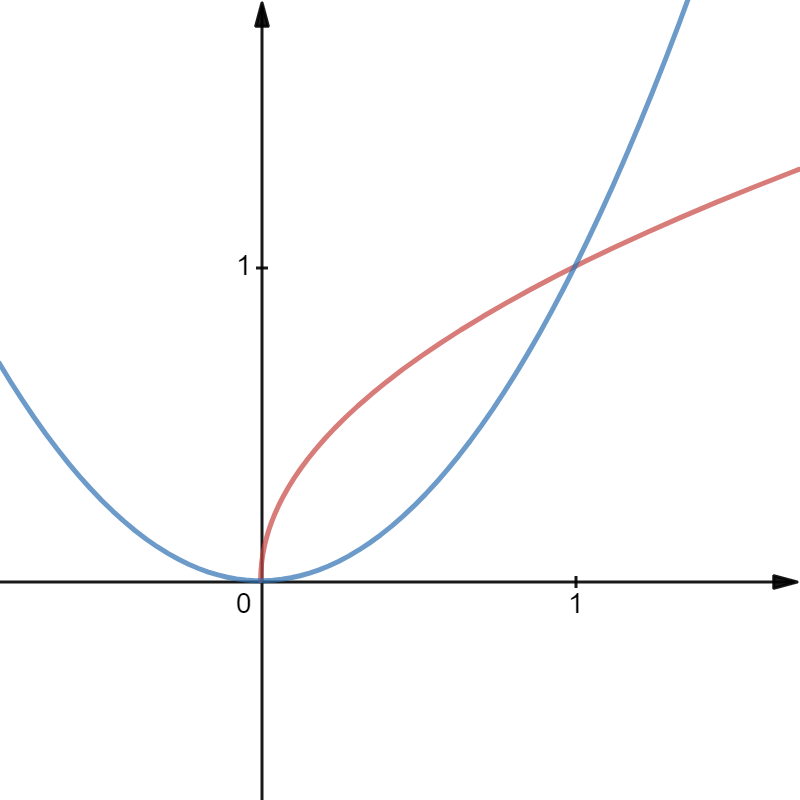
\includegraphics[scale=.3]{visualization.png}
        \caption{\textit{Graph of $y=\sqrt{x}$ and $y=x^2$.} Desmos link \href{https://www.desmos.com/calculator/xqjovtmzu0}{\textcolor{blue}{here}}, also see embed below.}
    \end{center}
\end{figure}
\begin{align}
    \intertext{We know that the formula for finding the volume using shells is}
    V                                                               & =2\pi\int_{a}^{b}\left(x\cdot f\left(x\right)\right)dx
    \intertext{Now lets try to create a formula finding the volume of an area bound by $2$ curves.}
    V                                                               & =2\pi\int_{a}^{b}\left(x\cdot f\left(x\right)\right)dx-2\pi\int_{a}^{b}\left(x\cdot g\left(x\right)\right)dx
    \intertext{This can be combined}
    V                                                               & =2\pi\int_{a}^{b}\left(x\cdot f\left(x\right)-x\cdot g\left(x\right)\right)dx
    \intertext{The $x$ can be factored out}
    V                                                               & =2\pi\int_{a}^{b}x\left(f\left(x\right)-g\left(x\right)\right)dx
    \intertext{Now find the difference between the top function and the bottom function to find the height of the cylinder. Looking at the graph,}
    \text{Upper}                                                    & = y = \sqrt{x}                                                                                                                                                           \\
    \text{Lower}                                                    & = y = x^2
    \intertext{Looking at the graph, the left bound is clearly $0$ and $1$}
    a                                                               & =\boxed{0}                                                                                                                                                               \\
    b                                                               & =\boxed{1}
    \intertext{Now plugin to the equation that we just made and integrate.}
    2\pi\int_{a}^{b}x\left(f\left(x\right)-g\left(x\right)\right)dx & =2\pi\int_{0}^{1}x\left(\left(\sqrt{x}\right)-\left(x^{2}\right)\right)dx                                                                                                \\
                                                                    & =2\pi\int_{0}^{1}x\left(x^{\frac{1}{2}}-x^{2}\right)dx                                                                                                                   \\
                                                                    & =2\pi\int_{0}^{1}\left(x^{\frac{3}{2}}-x^{3}\right)dx                                                                                                                    \\
                                                                    & =2\pi\left(\frac{2x^{\frac{5}{2}}}{5}-\frac{x^{4}}{4}\right)\Big|_{0}^{1}                                                                                                \\
                                                                    & =2\pi\left(\frac{2\left(1\right)^{\frac{5}{2}}}{5}-\frac{\left(1\right)^{4}}{4}-\left(\frac{2\left(0\right)^{\frac{5}{2}}}{5}-\frac{\left(0\right)^{4}}{4}\right)\right) \\
                                                                    & =2\pi\left(\frac{2\left(1\right)^{\frac{5}{2}}}{5}-\frac{\left(1\right)^{4}}{4}\right)                                                                                   \\
                                                                    & =2\pi\left(\frac{2}{5}-\frac{1}{4}\right)                                                                                                                                \\
                                                                    & =2\pi\left(\frac{3}{20}\right)                                                                                                                                           \\
                                                                    & =\frac{3\pi}{10}                                                                                                                                                         \\
                                                                    & \approx\boxed{0.942}
\end{align}
\end{document}